\subsection{Bottom hatch}
The bottom hatch, localized at the bottom of the arc chamber, has 80 cm
diameter, enabling mid-sized robots entry. As logistical challenge, the bottom
hatch is 10 m far from the blade and 4 m above the ground, thus the
system should be manually hoisted, transported on the slippery, cylindrical and
sloping arc chamber's floor and positioned near the blade. Using the bottom
hatch as the access for robot has the following advantages: large enough for
mid-sized robots, free access, it is normally used by operators to turbine
maintenance. And the following disadvantages: not large enough for large robots,
complex logistics to the hatch (scaffolding and hoists), difficulty for robot
moving and positioning in the arc chamber due to the slippery and sloping floor.

%Solutions for the bottom hatch have the following advantages and
%disadvantages:
%Soluções que utilizem o acesso pela escotilha inferior, de dimensão maior,
%apresentam as seguintes vantagens e desvantagens:

%\textbf{Advantages}:
%\begin{itemize}
%  \item large enough for medium sized robots
%  \item free access
%  \item it is normally used by operators to turbine maintenance.
%\end{itemize}

%\textbf{Disadvantages}
%\begin{itemize}
%  \item not large enough for large robots
%  \item complex logistics to the hatch. Scaffolding and hoists are
%  needed
%  \item difficulty for robot moving and positioning in the arc chamber due to
%  the slippery and sloping floor.
%\end{itemize}

%As logistical challenge, the bottom hatch, like all other accesses, is a
%logistical challenge and a common challenge of the metallization process. The
% bottom hatch has 80 mm diameter and is 4 m above ground. The system should be carried by a hoist
%manually operated, installed inside the arc chamber on scaffolding. The floor
%is slippery and has a cylindrical and inclined shape.

%O acesso pela escotilha inferior apresenta, como todos os outros
%acessos, um desafio logístico e o desafio comum do processo de metalização. O
%acesso à escotilha é realizado por uma abertura de 80 mm de diâmetro e 4 m
% acima do solo, logo os equipamentos são transportados por uma talha operada manualmente,
%instalada dentro do aro câmara, em andaimes. O solo é escorregadio e, devido à
%forma cilíndrica do aro câmara, curvilíneo e inclinado.

The system solutions is focused on mid-size manipulators, and modular base.
Solutions were divided into subsections in accordance with fixation strategies:
mobile robots that move on rails fixed on the blade; climbers; industrial
manipulators that move on rails fixed on the floor.

%Dessa forma, as soluções foram focadas em robôs de médio porte, peso reduzido
%devido ao transporte e às necessidades de movimentação e posicionamento do robô
%(trajeto escotilha à pá), e modular, quando possível.

%As soluções foram divididas em subseções de acordo com a fixação:
%robôs móveis que se locomovem em trilhos, robôs escaladores e manipuladores
%industriais com base fixa. 
%obs.:
%Colocar o robô entre as pás para aplicar revestimento de duas pás com uma
% instalação exige que o robô seja desmontado toda vez que a turbina for girada.
%Isso é ruim, pois após primeira aplicação a área fica de risco. Esta solução
%exige 5 movimentos no robô e 6 movimentos na turbina.

%A solução em que o robô fica atrás ou à frente exige que o robô seja
%movimentado apenas 2 vezes e a turbina fará 8 movimentos (duas voltas).

%TODO revisar todos os projetos sabendo as respostas
\subsubsection{Design of a mobile robot and rail fixed on blade}\label{proj_rail}
The concept solution of a robotic manipulator and rail base fixed on blade
satisfies all requirements for the HVOF coating and the inspection process. The
development of a compact system for easy transportation and its installation on the arc
chamber are possible, since the manipulator dimensions are reduced due to the
extra mobility provided by the rail.

%A utlização de um manipulador robótico sobre trilhos satisfaz todos os
%requisitos para a realização de um processo de inspeção e metalização
%utilizando a técnica HVOF. O desenvolvimento de um sistema compacto para o
%transporte através do acesso pela escotilha inferior e sua instalação no aro
%câmara da turbina são possíveis, pois as dimensões do manipulador podem ser
%reduzidas por meio da mobilidade extra proporcionada pela introdução do trilho.

In the context of the proposed application, the solution consists in a system
similar to Roboturb, presented in section \ref{sec::rail}. Thus the rail should
be flexible to be able to follow the blade curvature, it should allow several
placement options, and, as the blade is not ferromagnetic, the adhesion would
be by active suction cups with special material to work on large temperature
variations.

%No contexto da aplicação proposta, foram concebidas duas possibilidades para a
%fixação do sistema de trilhos. A primeira solução consiste em um sistema
%semelhante ao Roboturb, apresentado na seção \ref{sec::rail}. O sistema
% proposto se trata de um manipulador robótico com fixação diretamente na pá da
%turbina. O trilho deverá ser flexível para ser capaz de acompanhar a curvatura
%da pá e possibilitar diversas opções de posicionamento. Como o material da pá
%não possui alta permeabilidade magnética (Inox 420), a solução de fixação seria
%por ventosas ativas e com material específico para suportar as grandes
%variações de temperatura que a pá pode alcançar (temperatura ambiente a
%$100^oC$ durante a metalização).

%Uma abrangente pesquisa de robôs comerciais industriais de pequeno porte
% apontou que há manipuladores com carga entre 12 e 20 kg e velocidade necessários,
%sendo o LBR da Kuka o que possui melhor benefício peso/alcance, 30 Kg e 820 mm,
%respectivamente. %Para este manipulador, a metalização deverá ser
%realizada em, pelo menos, quatro etapas com quatro trilhos diferentes e
%customizados, e placas de sacrifício para evitar mau aplicação da metalização
%durante as trocas de sentido na movimentação do robô.

%A fixação de um trilho na pá apresenta diversas complexidades, como: a
%necessidade de manualmente instalar/desinstalar o sistema trilho/robô diversas
%vezes em cada pá; o projeto do trilho customizado e flexível; e ventosas ativas
%especiais que suportam variação de temperatura.




\textbf{Solution conclusion}

Fixing a rail on the blade has some complexities: rail and robot manual
installation/uninstallation for each blade side; design of customized flexible
rail; and design of special active suction cups for high temperature
variation. It is possible to use an industrial manipulator, such as the
Kuka lightweight (30 kg), making the design focused on signal processing,
mapping, localization, control, and the rail construction. 

%A solução com trilho externo se mostrou vantajosa em comparação ao robô em
%trilho customizado acoplado à pá, devido à complexidade e intervenções
%manuais. Há a possibilidade de utilizar um manipulador industrial, tornando o
%foco do projeto em processamento de sinais, mapeamento, localização e controle,
%além da construção do trilho. Porém, a montagem da estrutura e a instalação de
%todo o sistema atrás da pá podem ser custosas, sendo esta ainda uma solução
%considerada complexa.
\subsubsection{Design of robotic climbers}\label{proj_climbers}
In this subsection, the robotic solutions for HVOF coating are the fusion
of technologies documented in subsection~\ref{sota_climbers}. They will be an
adaptation of \emph{The Climber}, ICM, given their ability to reconfiguration.

%Nesta subseção, consideram-se soluções para HVOF de pás de turbinas robôs
%escaladores com fusão das tecnologias documentadas na
%seção~\ref{sota}, subseção~\ref{sota_climbers}. Será abordada uma versão
%adaptada do robô \emph{The Climber}, ICM, dado sua possibilidade de
%reconfiguração.

\emph{The Climber}, ICM, is a commercial solution which meets many
of the HVOF specifications and enables improvement without compromising its
structure. The robot's adhesion is suction type and the motion is flexible
mats.
The system has already been tested in hazardous environments, as wind turbines,
hydroelectric plants and others. We can divide the design into four systems:
mobility, adhesion, manipulator and autonomy.

%O robô \emph{The Climber}, ICM, é uma solução comercial que atende muitas das
%especificações HVOF e possibilita aperfeiçoamento sem comprometer sua
%estrutura. O robô possui sistema de adesão por sucção e locomoção através de
%esteiras flexíveis. O sistema já foi testado em ambientes de alta
%periculosidade, como turbinas eólicas, usinas hidrelétricas e outros. Podemos
%dividir o projeto em quatro sistemas: locomoção, adesão, manipulador e
% autonomia.

\emph{The Climber} uses only one vacuum chamber instead of the suction cups in
\cite{kim2008development}, for example. \emph{The Climber}'s flexible mats allow
smoothly and continuously motion. The solution with a single chamber seems more
advantageous, as the robot can move on curvatures up to 30 cm radius.

%O sistema desenvolvido em \cite{kim2008development} tem mecanismo de
%locomoção por esteiras e adesão por sucção. O sistema é composto por polias,
%correias de borracha, ventosas, válvulas para cada ventosa, motores DC para as
% polias, sistemas de controle para as válvulas e para os motores. \emph{The Climber}
%utiliza apenas uma câmara de vácuo, em vez de ventosas, e esteiras flexíveis
% que permitem maior suavidade e continuidade ao movimento. A solução por uma única
%câmara parece mais vantajosa, já que o robô consegue se locomover em curvaturas
%de até 30 cm de raio.

In the specific case of the HVOF process, a manipulator applies the coating 
while the robot travels along the blade. The robot locomotion on the blade rises
some design issues: the blade temperature during the procedure requires an
active suction chamber special material; and mats and suction chamber must
work on highly curved surface.

%No caso específico da aplicação HVOF, o processo é realizado com
%manipulador enquanto o robô percorre a pá da turbina. A locomoção do
%robô sob a pá levanta algumas questões de projeto: a
%temperatura da turbina durante o procedimento exige uma solução por câmara
% ativa de material especial; e como se comporta o robô em curvaturas
%acentuadas. 


In adhesion by suction, an intelligent security mechanism should be implemented,
with accelerometers, gyros and other sensors to ensure the shutdown of the
electronics and the supply of the HVOF gases in case of fall. The solution of a
mobile robot path planning increases safe operation and the optimal control of the adhesion
mechanism can limit the maximum suction force.

%Em sistemas de adesão por sucção, deve-se considerar um mecanismo
%inteligente de segurança, possivelmente utilizando acelerômetros e outros
%sensores, para garantir o desligamento do sistema eletrônico e o fornecimento
% de gáses. A solução de um robô móvel com planejamento de trajetória aumenta a
%segurança da operação e o controle ótimo do mecanismo de adesão pode limitar a
% força máxima de sucção.


%O manipulador a ser projetado para aplicação HVOF possui as seguintes
%características: é leve para não comprometer a adesão e equilíbrio do sistema
%móvel; rápido e preciso conforme requer a aplicação HVOF; modular, já
%que a operação será realizada in-situ, em espaço confinado;
%não possui grandes dimensões, pois o robô é móvel e pode
%percorrer a pá, porém deve ser suficiente para operar em pontos de
%difícil acesso à base e considerar a distância mínima (230 mm) entre pistola
%HVOF e pá; e é capaz de sustentar a carga e vibrações geradas pela
%pistola HVOF. 

% Climber's path planning solution should consider both the mobile base and the
% manipulator. The literature is fairly consolidated on robotic manipulators, and
% many of these problems are already settled and available, as developed in
% \cite{manzdevelopment}. 

%A solução de robôs escaladores exige planejamento de trajetórias tanto da base
%móvel, quanto ao controle de manipuladores. A literatura sobre
%manipuladores é bastante consolidada, sendo muitos dos problemas citados já
%resolvidos e disponíveis no mercado, como o desenvolvido em
%\cite{manzdevelopment}. Os menores manipuladores industriais que sustentam a
%carga do sistema de metalização possuem em torno de 30 a 50 kg. Portanto, o
%conjunto manipulador, pistola e cabos pode possuir de 50 a 80 kg de massa.

%A tecnologia que verifica a necessidade de
%revestimento, com sensores laser e ultrassom, e poderá indicar o \textbf{mapa
%ou apenas realizar um teste de sucesso/falha} \citep{escaler2006detection}.

% The mission control is the planning and execution of tasks. The motion and
% adhesion control should be synchronized, performing the path planning,
% obstacle avoidance and environmental mapping, through a set of sensors such as
% accelerometers and laser. The manipulator control can be kinematic by visual
% servoing or by structured environment. And a vehicle support system will be
% responsible for security, smooth operation and power management.

%O sistema autônomo de um robô móvel é a inteligência do robô. Ele abrange o
%controle de missão, ou seja, o planejamento e execução das tarefas em modo
%autônomo. A locomoção será realizada pelo controle dos motores em conjunto com
% o controle do sistema ativo de adesão por sucção, o planejamento de trajetória, desvio de
%obstáculos e mapeamento do ambiente, através de um conjunto de sensores, como
%laser e acelerômetros. O controle do manipulador poderá ser cinemático por
%servovisão ou pela estruturação do ambiente. E um sistema de suporte do veículo
%ficará responsável pela segurança, bom funcionamento e gerenciamento de
% potência do robô.




%As características descritas acima como solução de um robô escalador impede a
%troca automática entre pás. Um robô escalador com tecnologia de avanço
% pendurado por braços é uma solução muito custosa em termos de controle e estrutura
%mecânica. Outra solução seria um robô com locomoção por segmentos deslizantes,
%como o RRX3, e adesão por sucção, porém a flexibilidade exigida para a
% locomoção entre pás e a distância entre turbinas complexifica o projeto. Dessa forma, a
%troca entre pás deverá ser manual.

%\textbf{Versão adaptada Roboturb}

%O Roboturb, como já descrito na subseção~\ref{sec::rail}, é um
%manipulador que se locomove em um trilho, este acoplado à pá da turbina
%por ventosas (sucção). A solução não permite a extensão
%do manipulador, já que o peso desequilibra a estrutura e não há torque para
%compensar a força exercida no efetuador durante a operação HVOF. A segunda
%solução de robôs escaladores é adicionar um trilho perpendicular e transformar
%o Roboturb em um robô móvel, com locomoção através de dois trilhos, idéia
%semelhante ao \emph{Climbing robot for Grit Blasting}, que utiliza duas
%plataformas deslizantes com ventosas.

%Os trilhos são compostos por esteiras flexíveis nas extremidades para a
%locomoção, como \emph{The Climber}, e as ventosas são ativas e distribuídas por
%todo o trilho. O manipulador só necessitaria mover em um dos trilhos para
%percorrer toda a pá, já que os trilhos também se movimentam. 

%A solução de trilhos móveis com manipulador é dependente à curvatura da pá da
%turbina e o aumento da flexibilidade do trilho para se locomover sob a pá pode
%impedir a movimentação do manipulador. Dessa forma, é considerada uma solução
%muito específica e restrita à aplicação.

\paragraph{Solution conclusion}
Although tempting because of the autonomy, the surface complexity of the
turbine blade, the confined environment, and the required speed and payload are
major challenges to the design. 

The climber's manipulator would be complex and should have the
following characteristics: to be lightweight, avoiding base complex adhesion and
balance; to be fast and accurate as required by the HVOF application; to be
modular, as the operation is performed in confined spaces; to
be small, improving mobility, but capable to operate on blade's edges with 230
mm minimum distance; and to have high payload and vibration resistance. The
smaller industrial manipulators with required the payload weighs 30 to 50 kg.
Therefore, manipulator, HVOF gun and cables weighs 50 to 80 kg. The
manipulator greatly increases the dimensions of the mobile base and hence
diminishes their workspace, slowing the process.

Finally, the climber as described above does not switch automatically between
blades. A climber with arms to switch between blades is a costly solution in
terms of control and mechanical structure. Another solution would be a robot with
locomotion by sliding segments, as RRX3, and adhesion by suction, but the
flexibility required for motion between blades complicates the design. Thus,
the exchange between blades should be manual.

Compared to alternative solutions, a climber would be a general solution,
it has logistical advantages, but it is a robotic challenge. 

%Apesar de tentador devido à autonomia, a complexidade da estrutura da pá, o
%ambiente, a velocidade requerida e a carga do sistema de metalização são
%grandes desafios ao projeto. São estimados 50 kg de
%carga para o conjunto manipulador, cabos e pistola, o que aumenta muito as
%dimensões da base móvel e, consequentemente, diminui a sua área de atuação,
%tornando o processo mais demorado.
\subsubsection{Proposed solution}\label{proj_manip}

There are several industrial manipulators which fulfill the HVOF
requirements. Companies as Fanuc, Motoman, ABB and KUKA, for example,
manufacture manipulators compatible with the bottom hatch dimensions and HVOF
requirements, and workspace that the entire turbine blade could be coated at a
fixed base position. However, those manipulators are too big to operate behind
the blade, on the distributor side, due to environment collision, joint
constraints, and robot manipulability. Besides, manipulators with such
workspace are heavyweight, thus the robot placement and motion would be complex
inside the Runner area. A feasible solution would be to select a mid-sized
manipulator and made a rail base to place and move the robot.

%Há diversos manipuladores robóticos industriais com as especificações
%necessárias para a realização da tarefa de metalização por HVOF. As empresas
%Fanuc, Motoman, ABB e KUKA fabricam manipuladores com dimensões compatíveis com
% o acesso pela escotilha inferior e velocidade, precisão, e espaço de trabalho que
%cumprem os requisitos para a execução do processo em todo um lado da pá, em uma
%base fixa. Porém, há incompatibilidade atrás da pá e a necessidade de escolher
% a posição correta do manipulador em relação à pá, a fim de maximizar a sua área de trabalho, no ambiente da
%turbina, o que pode restringir os seus movimentos.
%Como as pás podem ser giradas até um ângulo de $14.5^o$, são discutidas as
% ideias de posicionamento do manipulador entre as pás, a fim de executar a operação em ambos os lados da
%pá (um lado de cada pá), e o posicionamento fixo à frente e depois atrás à pá.

The base consists of a transport rail and a positioning rail, both fixed
in the Runner area by magnetic coupling and/or welding. The first solves a
logistic problem, as it starts at the bottom hatch entry and goes to the blade,
moving the robot through the Runner area. The latter is coupled to the main rail and positions the robot close to the
blade, enabling displacement along it, solving the horizontal HVOF cover of the
blade.

The base may be summarized in three joints: prismatic (main rail), revolution
(joint between main and second rail), and prismatic (second rail) (P-R-P). As
the robot can not vertically cover the entire blade, there is still the need of
different vertical positions, which should be manually selected. The blade can
be coated on linear or circular motion, and, in both cases, the manipulator will
be responsible for speed, position and gun orientation. The solution for gun
direction exchange (\textit{long stop}) is an actuated valve to redirect the
coating particles.

%A base por um trilho de transporte e um de posicionamento. Ambos são fixados no
%aro câmara por acoplamentos magnéticos e/ou solda. O primeiro começa na
%entrada da pá e vai até a pá, permitindo o deslocamento do robô pelo aro
% câmara.
%O último é acoplado ao trilho principal e posiciona o robô próximo a pá, além
% de possibilitar o deslocamento ao longo desta. Dessa forma, a base pode ser
%resumida em três juntas: prismática, revolução e prismática (PRP). Como o robô
%não possui alcance de toda a pá, há, ainda, a necessidade de posições verticais
%diferentes escolhidas manualmente. A pá pode ser processada em movimentos
%circulares ou lineares e, em ambos os casos, o manipulador ficará responsável
% pela velocidade, posição e orientação do processo. A troca de sentido de movimento deverá ocorrer fora da
%pá, ou devem ser utilizadas placas de sacrifício, ou válvulas para
%redirecionamento das partículas de revestimento.

%Esse tipo de abordagem simplifica a movimentação do robô no
%trilho, uma vez que o trilho seria totalmente reto, e possibilitaria a
%metalização de um dos lados das quatro pás com uma única instalação de base.
%Porém, mesmo nesta solução, a altura do trilho deverá ser ajustada três vezes
% para cada lado de pá.


%Em ambos os sistemas propostos, é necessária a implementação de um sistema de
%localização do robô em relação à pá, tornando possível a geração de um
%planejamento de trajetórias para o processo de metalização. O sistema de
%localização pode ser concebido por sensores externos
%ao robô (câmeras e outros), ou instalados no próprio manipulador/base.


%The alternative to avoid contact with the blade consists of a single rail
%rectilinear fixed by magnetic bases or welding of the rim in the soil chamber.
% Like the robot has not reach all the shovel, there is still a need positions
%different vertical. The blade can be processed in circular movements or
%linear and, in both cases, the handler will be responsible for the speed,
%position and orientation of the process. The exchange direction of movement
% should occur outside the shovel or must sacrifice cards used.

%\paragraph{Transport rail}

A mid-sized robot manipulator should be hoisted through the bottom
hatch, placed on a rail base with magnetic holders and carried
to the blade, as in Fig.~\ref{fig::rail1}. At that position, the robot should
switch to the other rail. 
%That strategic position (robot between blades) is
% advantageous as it allows the manipulator to operate adjacent blades without
% rail disassembling or major positioning changes.

\begin{figure}[h!]	
	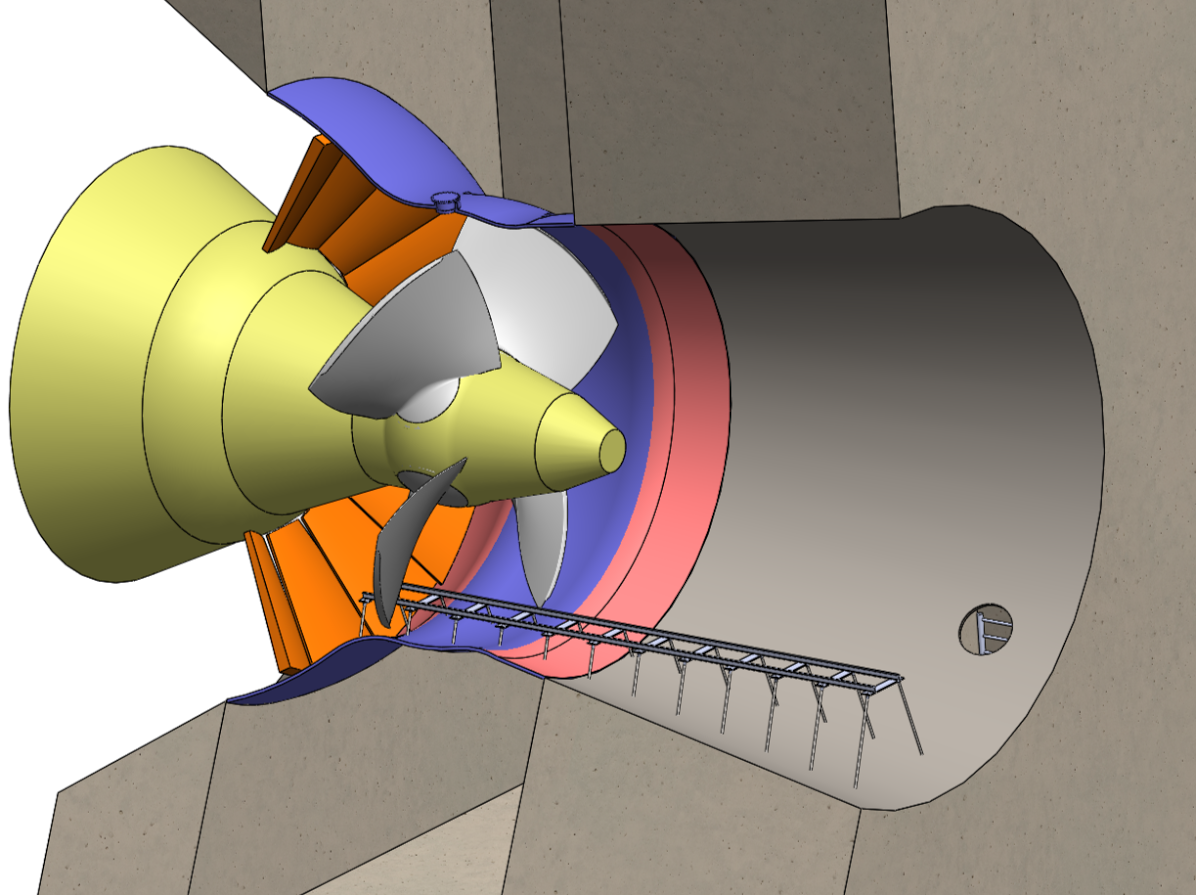
\includegraphics[width=\columnwidth]{figs/manipuladores/rail1.PNG}
	\caption{Transport rail mounted inside the turbine.}
	\label{fig::rail1}
\end{figure}

%A figura~\ref{fig::andaime} mostra o espaço entre as pás da turbina, dentro do
%aro câmara. Um robô manipulador de médio porte pode ser fixado em uma base
%magnética, na posição que se encontra a escada da figura~\ref{fig::andaime}.
%Essa posição é vantajosa por possibilitar a execução da tarefa em duas pás
%(frente de uma e verso da outra), sem desmontar ou fazer grandes alterações no
%posicionamento da base do robô, diminuindo as intervenções e tempo de tarefa.

% However, a purely geometric study shows that the necessary workspace for
% adjacent blades coating, assuming a fixed base between the blades,
% is around 5 m reach. The industrial manipulator IRB5500, for example, developed
% by ABB for painting, and is a large sized manipulator and has 3 meters range,
% 600 kg.
% As no mid-sized industrial robot was found for completely cover
% the blade on a fixed base position, a positioning rail should be made.

%O estudo puramente geométrico demonstra que o alcance do manipulador robótico
%para o processamento de ambos os lados das pás, considerando uma base fixa
% entre as pás, deverá ser em torno de 5 metros. O manipulador industrial IRB5500,
%desenvolvido pela ABB para pintura, possui 3 metros de alcance, porém 180 kg, o
% que já dificulta ou até impossibilita a logística de movimentação e posicionamento in-situ. Não foi encontrado um robô
%industrial com o alcance necessário e que tivesse as dimensões máximas da
%escotilha inferior. 

%A solução conceitual de posicionar um manipulador industrial entre as pás deve
%avaliar, portanto, todas as configurações necessárias da base (orientações e
%posições) para garantir que todo o espaço de trabalho do manipulador mais base
%cubra os lados de ambas as pás. O número de configurações e o projeto
%mecânico da base são necessários para a viabilização da solução,
%uma vez que será possível avaliar as intervenções e complexidades. Bases
%autônomas diminuem o número de intervenções e aumentam a precisção do sistema,
%porém aumentam a complexidade, o custo devido ao número de sensores e
% atuadores, e o peso do sistema, prejudicando a logística.

%\paragraph{Positioning rail}
Fixedly positioning a robotic manipulator with magnetic holders at the front or
at the back of the blade for HVOF process is a natural solution, since it is
similar to the companies procedure. However, a purely geometric
study, using the real dimensions of the blade, shows that the manipulator must
have more than 2.5 m reach for full blade cover. To perform this task, workspace
analysis was conducted to confirm the geometric study and a mid-sized
robot can not reach the entire blade. Therefore, its base should be able to move
horizontally and vertically (Fig.~\ref{fig::rail2}).

\begin{figure}[h!]	
	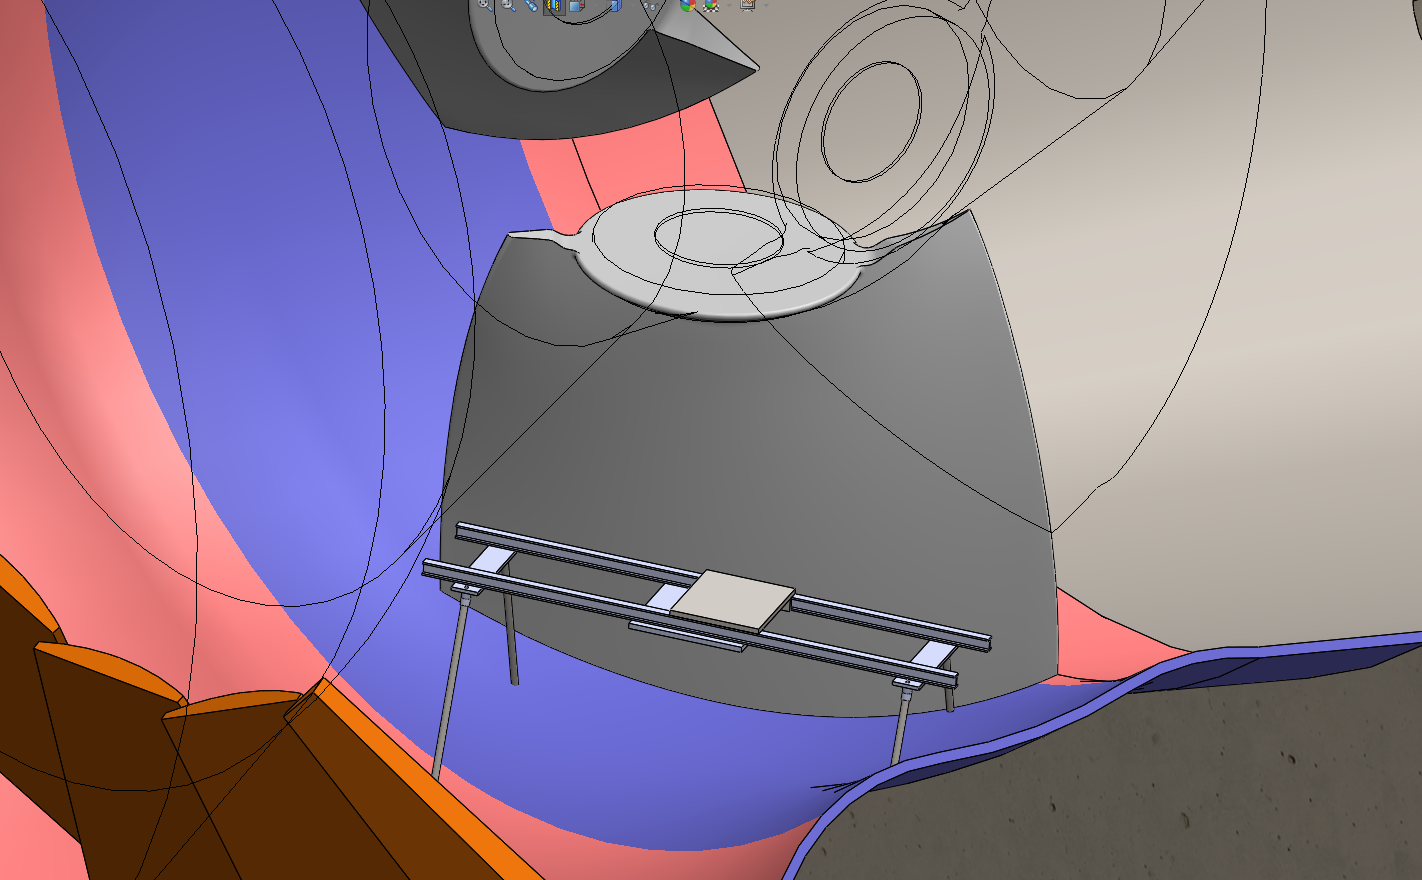
\includegraphics[width=\columnwidth]{figs/manipuladores/rail2.PNG}
	\caption{Positioning rail behind the blade.}
	\label{fig::rail2}
\end{figure}
%Posicionar de maneira fixa um manipulador com base magnética à frente e atrás
% da pá para a metalização é uma solução natural, já que é semelhante à utilizada pela
%empresa Rijeza atualmente. Um estudo puramente geométrico, utilizando as
%dimensões da pá, mostra que o manipulador deve possuir alcance de 1.7 m e ser
%posicionado a uma altura de 1.1 m em relação ao solo. Estudos de espaço de
%trabalho, manipulabilidade e colisões devem ser realizados para confirmar o
%estudo geométrico.

This design also requires the implementation of a localization/calibration
system, as the robot must know its location in relation to the blade for
autonomous operation. The localization requires external sensors, as cameras, a
3D laser for mapping, a point laser sensor installed on the manipulator's
end effector, and base odometry for position feedback.

In this solution, a robot placed on a rail type base, on the floor, can not coat
the blades on top, thus the turbine must be manually rotated and a new
calibration process should be done for each step.

%O posicionamento do sistema à frente ou atrás da pá exige
%intervenções para rotação da turbina e para o deslocamento do sistema. Em
% relação a um sistema com base autônoma entre as pás, o processo parece mais custoso em
%intervenções manuais e mais demorado, porém bem mais simples em termos de
%robótica.

\paragraph{Solution conclusion}
In terms of robotics, industrial manipulators on a rail base is the simplest
among all solutions for the bottom hatch. There is no mechanical design for the
manipulator, since it will be acquired in one of the aforementioned
manufacturers, but the mechanics will be responsible for the base design (rigid
and modular), the magnetic couplings, and logistics.

%In
%addition, the following steps should be done:
%manipulator control, data processing, calibration, path planning and UI.

%A utilização de manipuladores industriais é a mais simples, em termos de
%sistemas robóticos, dentre todas as soluções para o acesso pela escotilha
%inferior.

%Não há projeto mecânico do manipulador, já que este será adquirido em um dos
% fabricantes citados. As dificuldades mecânicas do projeto serão em relação à logística de posicionamento e movimentação do robô dentro do aro câmara, e no desenvolvimento de uma base,
%que pode ser autônoma. Além disso, o projeto fica responsável pelo controle do
%manipulador, processamento de dados que envolvem o HVOF, planejamento de
%trajetórias e UI.

%The main challenge is to build a rigid base and the locomotion of
%Equipment for the ring chamber. This conceptual design will be one of fronts to
%the feasibility study.

%Os desafios consistem na construção de uma base rígida e a locomoção dos
%equipamentos pelo aro câmara. Este projeto conceitual será uma das frentes para
%o estudo de viabilidade.
 
%% TODO Elael: Nosso projeto cabeado
\subsubsection{Robô Bipartido}

Esse conceito é uma cadeia de dois manipuladores conectados por um ponto de
apoio capaz de fixar-se à pá. O apoio serve como forma reduzir o torque
necessário nas juntas ao reduzir a alcance necessário para cada manipulador
individualmente.

Para facilitar futuras referências nesse texto, o braço robótico que se
apoia sobre o chão será chamado de primário, manipulador que parte dele de
secundário e o ponto de apoio entre eles, capaz de fixa-se à pá, será chamado de
fixador.

A pistola de metalização presa ao manipulador secundário deve ter
alcance sobre toda a pá da turbina. Para isso existe uma gama de pontos
necessários onde o fixador deve ser posicionado. Com esse intuito o
manipulador primário da cadeia precisa ser projetado para ter uma região de
trabalho com um alcance total sobre esses pontos. Para tal, informações precisas
sobre o formato das pás são necessárias.

Para viabilizar a solução, é necessário verificar quais são as soluções
possíveis para gerar a aderencia do fixador sobre à pá. As tecnologias mais
difundidas são por força magnética e por diferença de pressão (ventosa).
As maiores preocupações com o relação a adesão são a capacidade de carga do
método e a resistência do \textit{coating}. As soluções por magnetismo e
por ventosa afetam de maneira diferente as camadas do material ao qual se
aderem. Enquanto o magnetismo atrai ativamente o material ao qual prentende
aderir, a ventosa apenas reduz a pressão do ar na região onde ela se fixa. Ambas
as soluções possuem versões ativas e passivas, assim como uma gama de opções com
relação à capacidade de suportar carga. Logo, para essas soluções, a carga
necessária a ser suportada, o magnetismo do material, a resistência à baixa
pressão do \textit{coating} e os efeitos da atração magnética, também, sobre o
\textit{coating} são perguntas que devem ser respondidas.

O braço secundário deve ser projetado para atingir os requerimentos de
posicionamento e velocidade da pistola de metalização, porém a região sob o
fixador, certamente, não estará disponivel para receber o revestimento. Assim, a
possibilidade, ou os requisitos necessários, de mover o fixador para uma região
da pá recém metalizada deve ser vista analisada antes do robô bipartido ser
considerado uma possibilidade.

\subsection{Robô Pendurado} 
